\chapter{Design}
\section{User Interface Design}
In general, the backgrounds will be a darker colour with a lighter shade used to indicate where the buttons are. Most text will be white, with emphasised text in one of the three accent colours.
The title bar and menu bar will be Windows' default colour.
All elements of my interface will need to be user friendly, meaning the colours will have to contrast against each other.\\
\textit{Note: all colours have been omitted from diagrams as well as the exact controls used on the forms. Panel controls (which will contain the other controls) are represented by the blue boxes. The final layout of forms can be seen in Appendix \ref{app:ScreenshotsOfForms}}
\subsection{Main Menu}
\begin{figure}[H]
    \centering
    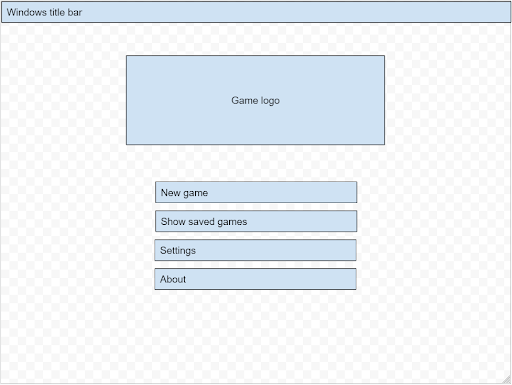
\includegraphics[width=0.7\textwidth]{images/design/mainMenu.png}
    \caption{Main menu design}
    \label{fig:design-mainMenu}
\end{figure}
This is the menu which will greet the character when they open the game. See the use case diagram for details of where each button leads.

\subsection{Main Game Screen}
\begin{figure}[H]
    \centering
    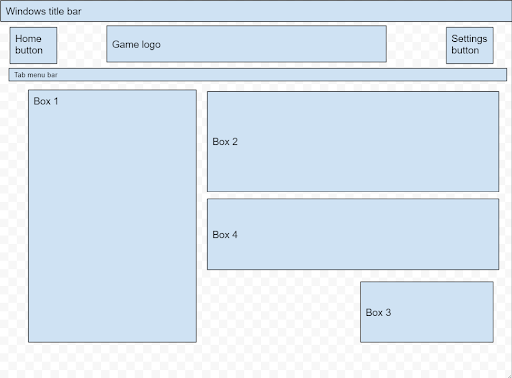
\includegraphics[width=0.7\textwidth]{images/design/mainGameScreen.png}
    \caption{Main game screen design}
    \label{fig:design-mainGameScreen}
\end{figure}
The general layout of all the following will remain the same for ease of use. All in their separate tabs (represented by the “Tab menu bar” underneath the Game logo).\\
If nothing is going in the box, then it will be left blank.\\
The home button will also act as a save progress button and prompt the user to say where they want their data saved to.

\subsubsection{Home tab}
Box 1 - TextBox control containing information about what has just happened in game (generated from the array of event objects).\\
Box 2 - Information about the character (including their name, age, current education situation).\\
Box 3 - Age up.\\
Box 4 - 

\subsubsection{Education tab}
Box 1 - Education events.\\
Box 2 - Information on current education situation.\\
Box 3 - Quit school.\\
Box 4 - 

\subsubsection{Jobs tab}
Box 1 - List of currently available jobs.\\
Box 2 - Information about the current job situation. \\
Box 3 - Quit job.\\
Box 4 - Options regarding new job.

\subsubsection{Crime tab}
Box 1 - Crime events.\\
Box 2 - \\
Box 3 - Commit random crime.\\
Box 4 - 

\subsubsection{Customise Character tab}
Box 1 - Editable attributes about the character.\\
Box 2 - End life.\\
Box 3 - Save button.\\
Box 4 - 

\subsubsection{Partners tab}
Box 1 - Available partners.\\
Box 2 - Actions about available partners.\\
Box 3 - \\
Box 4 - Information about current partner.

\subsection{Character Design Form}
\begin{figure}[H]
    \centering
    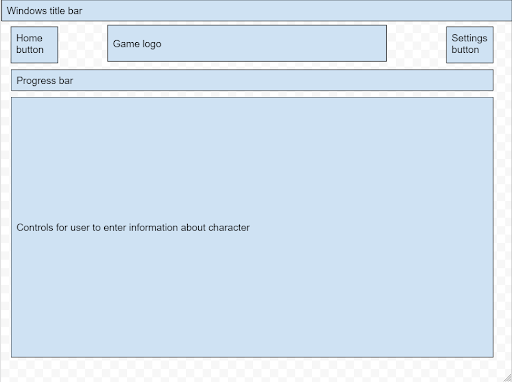
\includegraphics[width=0.7\textwidth]{images/design/characterDesigner.png}
    \caption{Character design form}
    \label{fig:design-characterDesigner}
\end{figure}
This will walk you through the steps required to create a new character. The controls on the form will change depending on the current step. 

\subsection{Choice Box}
\begin{figure}[H]
    \centering
    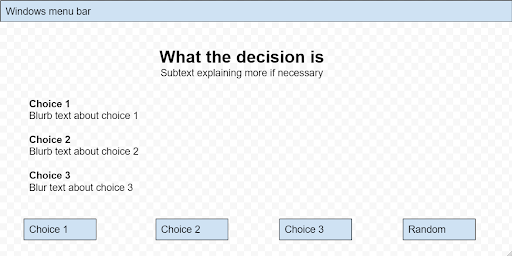
\includegraphics[width=0.7\textwidth]{images/design/choiceBox.png}
    \caption{Choice box form design}
    \label{fig:design-choiceBox}
\end{figure}
This will be a standard dialogue box (created in a form) which is generated each time there is a 3-way choice for the user to make. The random button will randomly select one of the three choices for the user. It will be the default 'ok' button (it is the button which is pressed when you press the enter key on the keyboard).

\subsection{Settings}
The settings menu will be accessible from within most of the forms of the app. Within it there will be accessibility options.

\subsection{Icons}
Icons will be downloaded from this \href{https://www.flaticon.com/}{Flaticon}.\\
Within the website, there is a colour change tool which can be used to change the colour of line icons. I will make use of this feature to make sure all of my icons are visable on the dark background.

\subsection{Fonts}
I will be using Segoe UI in the regular font face, with headings emphasised in bold and a larger size.

\subsection{Colours}
The background of my app will primarily be black, with dark grey buttons. 
\begin{table}[H]
\centering
\begin{tabularx}{0.8\textwidth}{llll}
\textbf{Where colour will be used} & \textbf{Sample} & \textbf{Hex code} & \textbf{RGB code} \\
\hline
App background & \cellcolor[HTML]{1F1F1F}{\color[HTML]{FFFFFF} Sample text} & \#1F1F1F & 31 31 31 \\
Buttons & \cellcolor[HTML]{666666}{\color[HTML]{FFFFFF} Sample text} & \#666666 & 102 102 102 \\
Accent 1 & \cellcolor[HTML]{64A4D1}{\color[HTML]{FFFFFF} Sample text} & \#64A4D1 & 100 164 209 \\
Accent 2 & \cellcolor[HTML]{A76CB3}{\color[HTML]{FFFFFF} Sample text} & \#A76CB3 & 167 108 179 \\
Accent 3 & \cellcolor[HTML]{F8639A}{\color[HTML]{FFFFFF} Sample text} & \#F8639A & 248 99 154
\end{tabularx}
    \caption{Outline of colours used in the app}
    \label{tab:colours}
\end{table}

\section{In-Game Events}
When playing the game, there are a series of events which will happen. The most important one is “ageing” up. This event will progress the game.
\subsection{Age up event}
This event will happen when the player clicks the age up button.\\
There are lots of random elements to this event which will generate the course of the game for the player.
\begin{figure}[H]
    \centering
    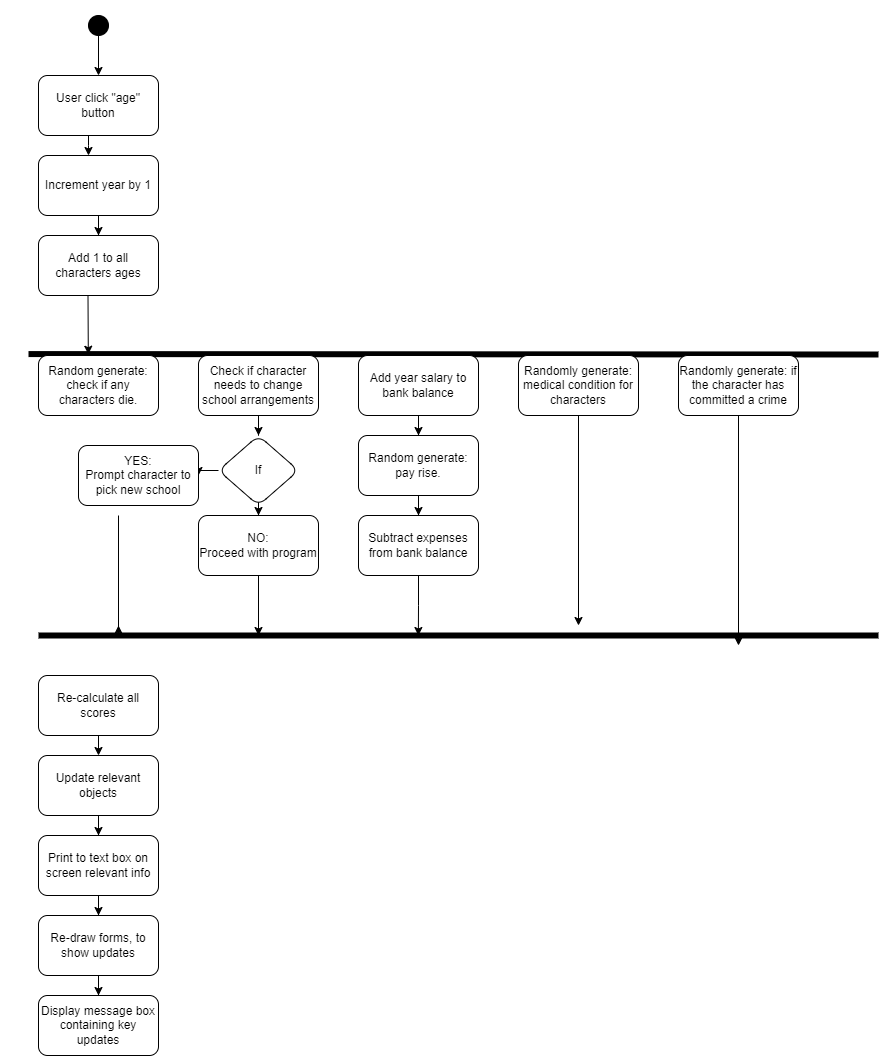
\includegraphics[width=0.9\textwidth]{images/design/ageUpEvent.png}
    \caption{Age up event}
    \label{fig:design-ageUpEvent}
\end{figure}

\subsection{Pre-Generated Events}
Most of the events in the game will be random, meaning each life which is played will have a random and fresh aspect to it. However, there will have to be a set of events which are randomly chosen from,  for example - crime (there will be a list of pre-decided crimes that can be randomly picked).

\section{Usability and Accessibility}
The settings menu will contain some accessibility options.\\
There will be no colour blind friendly options because the main colours of the game will contrast (light text on a darker background). Blues and pinks can sometimes be difficult for red/blue colourblind people to tell apart, as using RGB colours, pinks are achieved by mixing blue and red together. This shouldn’t be a problem in my game because even though I am using blues and pinks, they will never be used in critical parts of the game, only to emphasize or accent certain elements.\\
As this is a windows application, I will make sure to implement the correct tab order to allow people to navigate the entire application using only their keyboard or an on-screen keyboard.

\section{Class Diagrams}
Each attribute will have a get and set method within the class, this is something which C\# automatically implements for attributes. All other functions will be elsewhere in the code. Each class will also have a constructor, which will take inputs as parameters and construct the object.


\begin{figure} [H]
    \centering
    \begin{minipage}{0.45\textwidth}
        
    \end{minipage} \hfill
    \begin{minipage}{0.45\textwidth}
        
    \end{minipage}
\end{figure}

\subsection{Event}

\begin{figure} [H]
    \centering
    \begin{minipage}{0.45\textwidth}
        \begin{figure}[H]
        \centering
        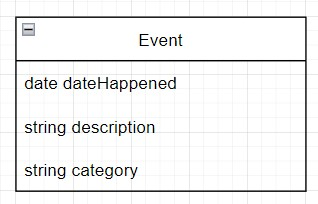
\includegraphics[width=0.9\textwidth]{images/design/class-event.jpg}
        \caption{Class diagram for Event}
        \label{fig:design-class-event}
        \end{figure}
    \end{minipage} \hfill
    \begin{minipage}{0.45\textwidth}
        The game will be based on events happening, these will be stored in an array of objects in the order in which they occurred. Events will be read-only as there will be no need to modify the event once it has occurred. The category will be used to categorise the events based on what type of events they are. This will allow the user to view only the crime related events for example.
    \end{minipage}
\end{figure}

\subsection{Score}

\begin{figure} [H]
    \centering
    \begin{minipage}{0.45\textwidth}
        \begin{figure}[H]
        \centering
        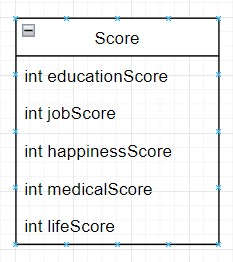
\includegraphics[width=0.9\textwidth]{images/design/class-score.jpg}
        \caption{Class diagram for Score}
        \label{fig:design-class-score}
        \end{figure}
    \end{minipage} \hfill
    \begin{minipage}{0.45\textwidth}
        This will be used for the main character to keep track of the scores which are key to the game.
    \end{minipage}
\end{figure}

\subsection{Job}

\begin{figure} [H]
    \centering
    \begin{minipage}{0.45\textwidth}
        \begin{figure}[H]
        \centering
        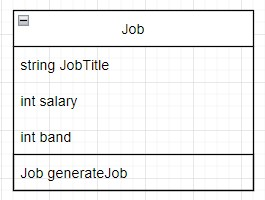
\includegraphics[width=0.9\textwidth]{images/design/class-job.jpg}
        \caption{Class diagram for Job}
        \label{fig:design-class-job}
        \end{figure}
    \end{minipage} \hfill
    \begin{minipage}{0.45\textwidth}
        There will be multiple uses of this class. One use will be to store the jobs which the game has generated that are available to the main character and the other use will be to store information about the main character's current job.
    \end{minipage}
\end{figure}

\subsection{ControlClass}

\begin{figure} [H]
    \centering
    \begin{minipage}{0.45\textwidth}
        \begin{figure}[H]
        \centering
        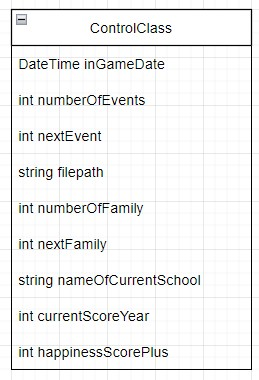
\includegraphics[width=0.9\textwidth]{images/design/class-controlClass.jpg}
        \caption{Class diagram for ControlClass}
        \label{fig:design-class-controlClass}
        \end{figure}
    \end{minipage} \hfill
    \begin{minipage}{0.45\textwidth}
    This class will be used to hold information about the current life in the game which means the program can easily manipulate data etc; for example, it stores the supporting information for the main character education element of the game.
    \end{minipage}
\end{figure}

\subsection{Person}

\begin{figure} [H]
    \centering
    \begin{minipage}{0.65\textwidth}
        \begin{figure}[H]
        \centering
        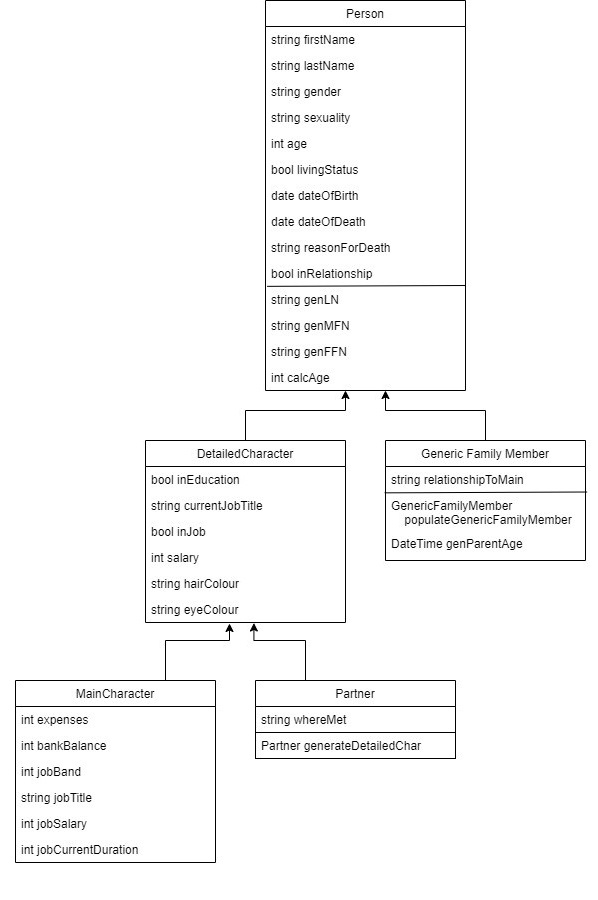
\includegraphics[width=0.9\textwidth]{images/design/class-person.jpg}
        \caption{Class diagram for Person}
        \label{fig:design-class-person}
        \end{figure}
    \end{minipage} \hfill
    \begin{minipage}{0.25\textwidth}
        This is the biggest group of classes, with the superclass person having many subclasses coming off of it. Having so many inherited classes means I can easily control all the aspects of the main character and partners\textquotesingle  life.
    \end{minipage}
\end{figure}

\section{Use Case Diagrams}
\begin{figure}[H]
    \centering
    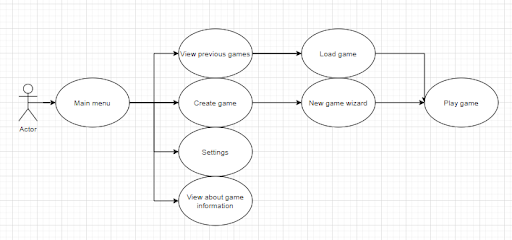
\includegraphics[width=0.8\textwidth]{images/design/useCaseDiagram.png}
    \caption{Use case diagram for the application}
    \label{fig:design-useCaseDiagram}
\end{figure}

\section{Algorithms}
A lot of my code isn’t suitable to be written in pseudocode because it uses lots of Visual Studios tools. For example - the character creations screen will make use of TextBox controls which are accessible by the name assigned; there is no way to write this in pseudocode, and the information from them would be passed into the constructor for the \verb|mainCharacter| class.
\subsection{Age-Up algorithm}
\begin{lstlisting}[style=pseudo]
on button press age up{
	stopProgress()
	gameDate = gameDate + 1 year
	mainCharacter.setAge(mainCharacter.getAge() + 1)
	ageCharacters()
	random = getRandom(1,10*randomModifier)
	if random == 1 then
		killCharacter(l)
	end if
	returned = checkSchoolChange()
	if returned == true then
		generateAndSelectSchools(mainCharacter.getAge)
	end if
	mainCharacterBank.setBalance(mainCharacterBank.getBalance + mainCharacter.getSalary)
	mainCharacter.setSalary(mainCharacter.getSalary + getRandom(0,1.5)
	mainCharacterBank.setBalance(mainCharacterBank.getBalance - mainCharacter.getExpenses)
	if random == 2 then
		generateMedicalConditionForOtherCharacters()
	end if
	if random == 3 then
		generateMedicalConditionForMainCharacter()
	end if
	if random == 4 then
		generateCrime()
	end if
	if random == 6 then
		generateCrime()
		generateMedicalConditionForMainCharacter()
		killOneCharacter()
	end if
	if random == 9 then
		killMainCharacter()
	end if
	updateScores()
	refillStoryBox()
	redrawForms()
	startProgress()
}
\end{lstlisting}

\subsubsection{Subroutines called from Age Up algorithm}

\noindent \textsc{Age all characters algorithm}\\
\verb|ageCharacters()|\\
This algorithm will age all the characters apart from the main character by one year. It will also need to make sure that none of the characters are getting too old and if they are change the probability of them dying, to increase the chance of this happening.
It will work by using a for loop to loop through all the elements in the characters array, getting their age then setting it to their age plus 1.\\

\noindent \textsc{Kill one character algorithm}\\
\verb|killCharacter(int numberToKill)|\\
This will randomly select a character from the array of character objects and kill one of them. If the number passed into it is greater than one then the subroutine will loop around again, killing more than one character. It will generate an event object containing this.\\

\noindent \textsc{Get random number}\\
\verb|getRandom(int bottom, int top)|\\
This subroutine will generate a random number between the two numbers specified as parameters.\\

\noindent \textsc{Check if the main character is due to change schools}\\
\verb|checkSchoolChange()|\\
This will get the main character\textquotesingle s age then check if it is one of the ages where a change of school is needed. If a change of school is needed, then it will return true, if not, it’ll return false.\\

\noindent \textsc{Generate new schools and select which one to go to}\\
\verb|generateAndSelectSchools()|\\
This will call the \verb|openFile(schools)| function, then loop through a pick 3 of the appropriate aged schools and open the 3-way choice box. It will then take the returned value from the 3-way choice box and update relevant attributes in the main character\textquotesingle s object. It will then generate an event object containing information from this.\\

\noindent \textsc{Generate medical condition}\\
\verb|generateMedicalConditionForOtherCharacters()|\\
\verb|generateMedicalConditionForMainCharacter()|\\
These two functions will work in the same way, just for different characters. They both will open the file containing the list of medical conditions, and randomly select one. The main character function will add it to the main character and the other characters one will randomly generate an index in the array of other characters to apply the medical condition to. For both of these, an event object will be generated.\\

\noindent \textsc{Generate and commit a crime}\\
\verb|generateCrime()|\\
This will open the file containing a crime and then randomly select one to be committed by the main character. Crimes will have their name and a severity scale next to them in the file, this means that the program can generate an appropriate punishment for the character. Both of these will be bundled up in an event object.\\

\noindent \textsc{Killing}\\
\verb|killOneCharacter()|\\
\verb|killMainCharacter()|\\
These will work in basically the same way, differing by who they kill. The kill one character will randomly generate a number which is the index in the array in which the person who is going to be killed can be found, then set their status to dead and change the death date to the current in-game date. The kill main character function will change the game state to game over, which will grey out all controls on the form and bring up a game over screen. \\

\noindent \textsc{Update the scores}\\
\verb|updateScores()|\\
This will recalculate all the scores in the game, and re-balance the weightings to best reflect what has just happened in the age.\\

\noindent \textsc{Refill the story box}\\
\verb|refillStoryBox()|\\
This will loop through the array of event objects and re-fill the TextBox which contains the life events.\\

\noindent \textsc{Redraw the forms}\\
\verb|redrawForms()|\\
This will be a standard function used which will re-draw the forms in c\# to make sure controls have all the correct data in them.\\

\noindent \textsc{Stopping Progress}\\
\verb|stopProgress()|\\
This will stop progress through the game by disabling the buttons which allow progress to happen.\\

\noindent \textsc{Starting progress}\\
\verb|startProgress()|\\
This will restart progress through the game by enabling the buttons which allow progress to happen.\\

\subsection{Choice Box Algorithm}
\begin{figure}[H]
    \centering
    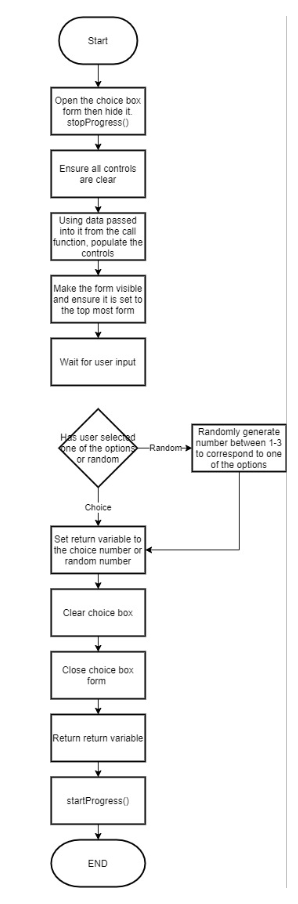
\includegraphics[width=0.4\textwidth]{images/design/choiceBoxAlgorithm.png}
    \caption{Algorithm for the choice box represented as a flowchart}
    \label{fig:design-choiceBoxAlgorithm}
\end{figure}
